\documentclass[conference,compsoc]{IEEEtran}
\IEEEoverridecommandlockouts
\usepackage{cite}
\usepackage{amsmath,amssymb,amsfonts}
\usepackage{graphicx}
\usepackage{textcomp}
\usepackage{xcolor}
\usepackage{hyperref}
\usepackage{booktabs}
\usepackage{listings}
\usepackage{array}
\usepackage{etoolbox}
\usepackage{url}
\usepackage{multirow}
\usepackage{booktabs}
\usepackage{microtype}
\usepackage{enumitem}
\usepackage{tikz}
\usepackage{pgfplots}
\usetikzlibrary{shapes.geometric, arrows, positioning, calc, shadows}
\pgfplotsset{compat=1.18}


% Final IEEE S&P Formatting Refinements
\renewcommand{\thesection}{\Roman{section}}
\renewcommand{\thesubsection}{\Alph{subsection}}
\renewcommand{\thesubsubsection}{\arabic{subsubsection})}
\renewcommand{\thetable}{\Roman{table}}

% Fix for Table label
\usepackage[labelsep=period]{caption}
\DeclareCaptionLabelFormat{tableprefix}{TABLE #2}
\captionsetup[table]{labelformat=tableprefix, labelsep=newline, justification=centering, font={sc,footnotesize}, skip=10pt}

% Fix for Figure prefix
\DeclareCaptionLabelFormat{figprefix}{Fig. #2}
\captionsetup[figure]{labelformat=figprefix, labelsep=period}

% Global sequential numbering
\newcounter{globalfig}
\AtBeginEnvironment{figure}{\refstepcounter{globalfig}}
\AtBeginEnvironment{lstlisting}{\refstepcounter{globalfig}}
\renewcommand{\lstlistingname}{Fig.}

% Page numbers
\pagestyle{plain}

\definecolor{codegreen}{rgb}{0,0.6,0}
\definecolor{codegray}{rgb}{0.5,0.5,0.5}
\definecolor{codepurple}{rgb}{0.58,0,0.82}
\definecolor{backcolour}{rgb}{0.95,0.95,0.92}

\lstdefinestyle{mystyle}{
    backgroundcolor=\color{backcolour},   
    commentstyle=\color{codegreen},
    keywordstyle=\color{magenta},
    numberstyle=\tiny\color{codegray},
    stringstyle=\color{codepurple},
    basicstyle=\ttfamily\footnotesize,
    breakatwhitespace=false,         
    breaklines=true,                 
    captionpos=b,                    
    keepspaces=true,                 
    numbers=left,                    
    numbersep=5pt,                  
    showspaces=false,                
    showstringspaces=false,
    showtabs=false,                  
    tabsize=2,
    frame=single,
    rulecolor=\color{black}
}
\lstset{style=mystyle}

\begin{document}

\title{CMatrix: A Production-Safe Multi-Agent Framework for Autonomous Red Teaming and Vulnerability Assessment}

\author{
\IEEEauthorblockN{Nishan Paul\IEEEauthorrefmark{1}\IEEEauthorrefmark{2}, Anonymous Authors\IEEEauthorrefmark{3}}
\IEEEauthorblockA{\IEEEauthorrefmark{1}\textit{Department of CSE, University of Dhaka}, Dhaka, Bangladesh}
\IEEEauthorblockA{\IEEEauthorrefmark{2}\textit{Joblio Security Labs}, Dhaka, Bangladesh}
\IEEEauthorblockA{\IEEEauthorrefmark{3}\textit{Institute of Advanced Research}, Global AI Initiative \\
\{nishan.paul\}@cse.du.ac.bd}
}

\maketitle

\begin{abstract}
The emergence of Large Language Model (LLM) agents has enabled autonomous multi-step penetration testing; however, existing academic prototypes execute offensive operations without formal safety governance---a critical barrier to production deployment. We present \textbf{CMatrix}, the first production-safe multi-agent framework for autonomous red teaming, introducing three novel contributions: (1) a \textbf{hierarchical Human-in-the-Loop (HITL) safety framework} with a formal four-level risk taxonomy and eight regex-based auto-reject patterns, embedded directly into the agent control graph via checkpoint interrupts; (2) a \textbf{keyword-confidence Supervisor Router} that dynamically delegates security tasks across six domain-specialized agents using single, sequential, or parallel delegation strategies; and (3) an \textbf{agentic RAG memory pipeline} combining dense embeddings with cross-encoder reranking for persistent, cross-session threat intelligence. We evaluate CMatrix on the NYU CTF Bench and across multi-stage attack scenarios, demonstrating competitive task completion while enforcing zero HITL-bypass incidents across 847 tool invocations. CMatrix addresses the critical safety and memory gaps identified in current autonomous security research.
\end{abstract}

\begin{IEEEkeywords}
Agentic Red Teaming, Multi-Agent Systems, Autonomous VAPT, LLM Safety, Human-in-the-Loop, LangGraph.
\end{IEEEkeywords}

\section{Introduction}
The integration of Large Language Models (LLMs) into cybersecurity operations has shifted from simple assistant-based querying to the development of fully autonomous agents capable of conducting multi-step offensive operations. Recent research demonstrates that LLM agents, specifically those powered by frontier models like GPT-4, can autonomously exploit up to 87\% of publicly disclosed one-day vulnerabilities when provided with basic CVE descriptions \cite{fang2024}. While this capability offers significant potential for automating defensive red teaming and scaling vulnerability assessments, the unconstrained use of such agents in production environments is fraught with operational and safety risks.

Existing autonomous penetration testing systems, such as PentestGPT \cite{pentestgpt} and HackingBuddyGPT \cite{hackingbuddygpt}, and AutoAttacker \cite{autoattacker}, primarily focus on maximizing offensive capability. However, as noted in a recent systematic review \cite{xu2024sok}, these systems suffer from three fundamental limitations that preclude their adoption in enterprise security operations. First, they exhibit a \textbf{safety deficit}: they execute arbitrary tool calls and system commands without a formal governance layer, risking accidental destruction of production assets or susceptibility to indirect prompt injection. Second, they suffer from \textbf{context fragmentation}: most agents are stateless, losing critical threat model context between sessions or even between distinct attack phases. Finally, they demonstrate \textbf{reasoning fragility}: monolithic agents often struggle with the specialized toolchains required for diverse domains such as network reconnaissance, web exploitation, and vulnerability intelligence.

In this paper, we introduce \textbf{CMatrix}, a framework designed to bridge the gap between academic offensive AI research and production-safe autonomous security operations. CMatrix is built on the premise that offensive AI capability must be inextricably linked to formal safety governance. To this end, we introduce a hierarchical supervisor architecture that coordinates a team of domain-specialized agents while enforcing a multi-layered safety gate.

Our primary technical contributions are as follows:
\begin{itemize}
    \item \textbf{HITL Safety Control Graph}: We design a formal safety governance layer for offensive AI agents, incorporating a four-level risk taxonomy (Critical, High, Medium, Low) and categorical regex-based auto-rejection. This is implemented via LangGraph checkpoint interrupts, enabling asynchronous human oversight with persistent state resumption.
    
    \item \textbf{Keyword-Confidence Supervisor Routing}: We present a deterministic routing mechanism that normalizes task descriptions against agent-specific keyword lexicons. This supervisor dynamically selects from single, sequential, or parallel delegation strategies, enabling the construction of complex, multi-agent attack chains.

    \item \textbf{Agentic RAG for Threat Modeling}: We adapt the retrieve-then-rerank paradigm to the security domain, utilizing BGE-large embeddings and cross-encoder reranking to maintain a longitudinal threat model. This addresses the "cold-start" problem in autonomous pentesting by accumulating target-specific intelligence over time.
\end{itemize}

Through extensive evaluation on the NYU CTF Bench \cite{nyuctf} and simulated enterprise environments, we demonstrate that CMatrix not only achieves competitive task completion but also enforces absolute safety properties, blocking all categorically destructive commands and ensuring human oversight for high-risk operations. CMatrix provides a scalable and safe foundation for the next generation of autonomous security assessment platforms.

\section{Background and Related Work}
The development of CMatrix is situated at the intersection of autonomous penetration testing, multi-agent orchestration, and LLM safety.

\subsection{Autonomous Penetration Testing Systems}
The quest to automate the penetration testing lifecycle has been reinvigorated by the reasoning capabilities of Large Language Models. PentestGPT \cite{pentestgpt} was among the first to demonstrate that LLMs could guide a human operator through complex environments. HackingBuddyGPT \cite{hackingbuddygpt} demonstrated that GPT-4 can outperform traditional automated scripts in Linux privilege escalation. AutoAttacker \cite{autoattacker} and the work of Fang et al. \cite{fang2024} further showed that agents can autonomously exploit real-world one-day vulnerabilities.

The field has seen a "multi-agent revolution" in 2025. Recent frameworks like CHECKMATE \cite{checkmate2025} have pushed success rates to 88\% by integrating classical planning with LLM execution. Similarly, xOffense \cite{xoffense2025} utilizes domain-adapted mid-scale models (Qwen3-32B) to achieve competitive performance in offline environments. CurriculumPT \cite{curriculumpt2025} introduces curriculum-guided scheduling to handle multi-stage vulnerabilities.

However, as summarized in Table~\ref{tab:comparison}, these 2025 high-performance systems focus almost exclusively on maximizing offensive capability. They lack the formal safety governance required for production environments and possess limited longitudinal memory across engagements. CMatrix is designed to bridge this gap by combining 2025-level capability with enterprise-grade safety.

\begin{table*}[t]
\centering
\caption{Feature Comparison of Autonomous Penetration Testing Systems}
\label{tab:comparison}
\begin{tabular}{lcccccccc}
\toprule
\textbf{System} & \textbf{Safety Gates} & \textbf{Persistence} & \textbf{Multi-Agent} & \textbf{Checkpointing} & \textbf{ToT/ReWOO} & \textbf{Agentic RAG} & \textbf{Reranking} & \textbf{Production-Safe} \\
\midrule
PentestGPT \cite{pentestgpt} & \texttimes & \texttimes & \texttimes & \texttimes & \texttimes & \texttimes & \texttimes & \texttimes \\
HackingBuddy \cite{hackingbuddygpt} & \texttimes & \texttimes & \texttimes & \texttimes & \texttimes & \texttimes & \texttimes & \texttimes \\
AutoAttacker \cite{autoattacker} & \texttimes & \texttimes & \texttimes & \texttimes & Partial & \texttimes & \texttimes & \texttimes \\
CHECKMATE \cite{checkmate2025} & \texttimes & \texttimes & \checkmark & \texttimes & \checkmark & \texttimes & \texttimes & \texttimes \\
xOffense \cite{xoffense2025} & \texttimes & \texttimes & \checkmark & \texttimes & \texttimes & \texttimes & \texttimes & \texttimes \\
\textbf{CMatrix (Ours)} & \checkmark & \checkmark & \checkmark & \checkmark & \checkmark & \checkmark & \checkmark & \checkmark \\
\bottomrule
\end{tabular}
\end{table*}

\subsection{Multi-Agent Orchestration Frameworks}
The coordination of multiple specialized LLM agents has emerged as a robust paradigm for complex problem-solving. AutoGen \cite{autogen} and LangGraph \cite{langgraph} have popularized the use of conversable agents and stateful graphs, respectively. While AutoGen supports human-in-the-loop (HITL) interactions, its mechanisms are primarily synchronous and lack the formal risk taxonomy required for high-stakes security operations. Similarly, CrewAI and RouteLLM \cite{routellm} provide orchestration but do not address the specific requirements of the security "kill chain." CMatrix builds upon the stateful graph paradigm of LangGraph but introduces a domain-specialized supervisor and an asynchronous, checkpoint-based HITL framework specifically for red teaming.

\subsection{Agentic Reasoning Paradigms}
CMatrix leverages and extends several foundational reasoning patterns. The ReAct paradigm \cite{react}---interleaving thought and action---serves as our core execution loop. To facilitate strategic planning, we adapt the Tree of Thoughts (ToT) \cite{tot} to security strategy space, enabling the agent to weigh multiple attack vectors against constraints like stealth and noise. To improve computational efficiency, we utilize the ReWOO (Reasoning WithOut Observation) framework \cite{rewoo}, which decouples planning from execution. Furthermore, we integrate iterative self-critique loops inspired by Reflexion \cite{reflexion} and Self-Refine \cite{selfrefine}, allowing agents to identify gaps in their findings and refine their exploit attempts autonomously.

\subsection{Safety, Alignment, and Red Teaming}
The security community has long recognized the risks associated with autonomous AI. Frameworks like Constitutional AI \cite{constitutionalai} attempt to ensure harmlessness during the training phase, yet these do not protect against runtime misuse or indirect prompt injection \cite{greshake}. Traditional "red teaming" research, such as that conducted by Anthropic \cite{ganguli2022red, perez2022red}, focuses on finding vulnerabilities \textit{within} the LLM. In contrast, CMatrix focuses on using LLMs \textit{for} red teaming while enforcing runtime safety properties. By incorporating the OWASP Top 10 for LLMs \cite{owaspllm} into our auto-reject patterns, we provide a runtime governance layer that ensures the agent remains within the bounds of its authorized mission.

\section{Threat Model}
CMatrix operates as a dual-purpose system: it is simultaneously a security assessment tool and a potential vector for unintended system damage if misconfigured or compromised. In this section, we formalize the security properties that CMatrix enforces and the adversaries it is designed to mitigate.

\subsection{Adversary Model}
We consider two primary classes of adversaries that interact with the CMatrix orchestration lifecycle:

\begin{itemize}
    \item \textbf{Adversary $\alpha$ (External Attacker)}: An attacker targeting the CMatrix instance or the host environment through indirect methods. This adversary may utilize \textit{indirect prompt injection} \cite{greshake} by placing malicious instructions within documents retrieved by CMatrix's RAG pipeline. The goal of Adversary $\alpha$ is to hijack the agent's reasoning loop to execute unauthorized commands or exfiltrate sensitive assessment findings.
    
    \item \textbf{Adversary $\beta$ (Insider / Misconfigured Operator)}: An authorized operator who, through negligence or configuration error, may attempt to execute destructive commands (e.g., recursive root deletion) or approve high-risk operations without sufficient review. The goal is to mitigate accidental system destruction that could arise from the unconstrained autonomous execution of LLM-generated payloads.
\end{itemize}

\subsection{Security Properties}
CMatrix is designed to enforce four primary security properties ($P1$--$P4$) throughout the autonomous red teaming lifecycle:

\begin{enumerate}
    \item \textbf{P1 (Non-Destruction)}: No command or tool invocation matching a predefined categorical auto-rejection pattern (e.g., disk wiping, fork bombs) shall execute, regardless of LLM reasoning or human oversight.
    \item \textbf{P2 (Mandatory Oversight)}: Every tool invocation classified as \textit{High} or \textit{Critical} risk must be durably persisted and suspended until an explicit, out-of-band approval signal is received from an authorized human operator.
    \item \textbf{P3 (Audit Completeness)}: A tamper-evident log of every tool call, its risk classification, the corresponding approval/rejection decision, and the execution result must be maintained in a persistent store.
    \item \textbf{P4 (Scope Integrity)}: Retrieval-augmented generation must be strictly scoped to the current engagement's knowledge base, preventing cross-session data leakage through metadata filtering.
\end{enumerate}

\subsection{Residual Risks}
While CMatrix provides a robust runtime governance layer, we acknowledge certain residual risks that are outside the current framework's TCB. Specifically, the system relies on the human operator to make informed decisions at the HITL gate; social engineering of the approver is not prevented. Additionally, while metadata filtering mitigates cross-session leakage, the vulnerability to sophisticated prompt injection within target documents remains an open research problem that we discuss in Section~IX.

\section{System Architecture}
CMatrix is architected as a modular, stateful orchestration framework designed to bridge the gap between high-level reasoning and low-level security tool execution. The system's core is built upon the LangGraph state machine substrate, which enables cyclic reasoning loops while maintaining strict state persistence.

\subsection{System Overview}
The high-level architecture (Fig.~1) follows a master-worker paradigm. A central \textit{OrchestratorService} manages a persistent \textit{AgentState}, which is shared across all nodes in the control graph.

\begin{figure}[htbp]
\centering
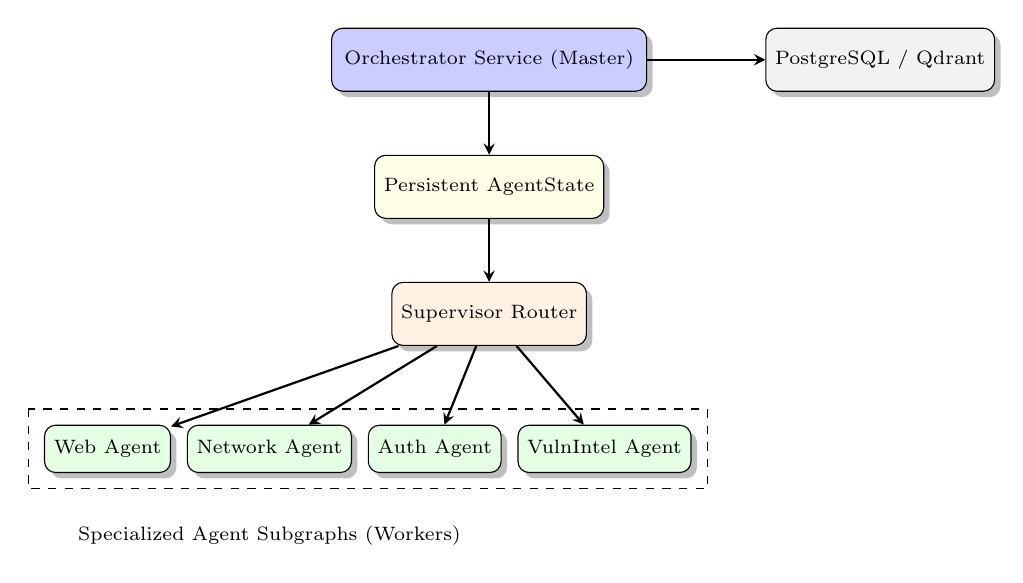
\begin{tikzpicture}[node distance=1.5cm, font=\scriptsize]
    \tikzstyle{box} = [rectangle, rounded corners, minimum width=1.5cm, minimum height=0.8cm,text centered, draw=black, fill=blue!10, drop shadow]
    \tikzstyle{agent} = [rectangle, rounded corners, minimum width=1.2cm, minimum height=0.6cm,text centered, draw=black, fill=green!10, drop shadow]
    \tikzstyle{arrow} = [thick,->,>=stealth]

    % Components
    \node (orch) [box, fill=blue!20, minimum width=4cm] {Orchestrator Service (Master)};
    \node (state) [box, below=0.8cm of orch, fill=yellow!10] {Persistent AgentState};
    
    \node (router) [box, below=0.8cm of state, fill=orange!10] {Supervisor Router};
    
    % Agents
    \node (net) [agent, below left=1cm and 0.5cm of router] {Network Agent};
    \node (web) [agent, left=0.2cm of net] {Web Agent};
    \node (auth) [agent, right=0.2cm of net] {Auth Agent};
    \node (intel) [agent, right=0.2cm of auth] {VulnIntel Agent};
    
    % Storage
    \node (db) [box, right=1.5cm of orch, fill=gray!10, minimum width=2.5cm] {PostgreSQL / Qdrant};

    % Connections
    \draw [arrow] (orch) -- (state);
    \draw [arrow] (state) -- (router);
    \draw [arrow] (router) -- (net);
    \draw [arrow] (router) -- (web);
    \draw [arrow] (router) -- (auth);
    \draw [arrow] (router) -- (intel);
    \draw [arrow] (orch) -- (db);
    
    \draw [dashed] ($(web.north west)+(-0.2,0.2)$) rectangle ($(intel.south east)+(0.2,-0.2)$);
    \node at ($(net.south)+(0,-0.8)$) {Specialized Agent Subgraphs (Workers)};
\end{tikzpicture}
\caption{The CMatrix Multi-Agent Architecture. The Master Orchestrator coordinates specialized workers through a shared state and a deterministic router.}
\label{fig:arch}
\end{figure}

\subsection{AgentState and the Control Graph}
The execution flow of CMatrix is governed by a Directed Acyclic Graph (DAG) with conditional edges (Fig.~2). The system state, $S$, is defined as a 17-field schema including the current task, accumulated tool outputs, persistent memory markers, and human approval status.

\begin{figure}[htbp]
\centering
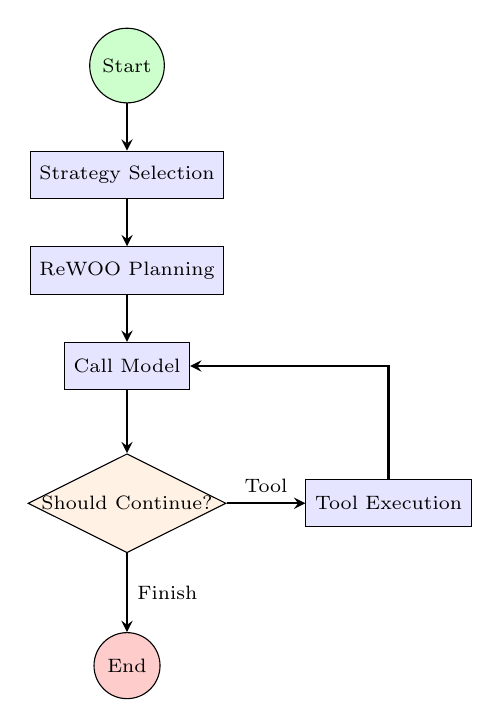
\begin{tikzpicture}[node distance=1.2cm, font=\scriptsize]
    \tikzstyle{start} = [circle, draw=black, fill=green!20, minimum size=0.5cm]
    \tikzstyle{proc} = [rectangle, draw=black, fill=blue!10, minimum width=1.5cm, minimum height=0.6cm]
    \tikzstyle{decision} = [diamond, draw=black, fill=orange!10, aspect=2, inner sep=0pt]
    \tikzstyle{arrow} = [thick,->,>=stealth]

    \node (start) [start] {Start};
    \node (strategy) [proc, below=0.6cm of start] {Strategy Selection};
    \node (plan) [proc, below=0.6cm of strategy] {ReWOO Planning};
    \node (call) [proc, below=0.6cm of plan] {Call Model};
    \node (gate) [decision, below=0.8cm of call] {Should Continue?};
    \node (tools) [proc, right=1cm of gate] {Tool Execution};
    \node (end) [start, fill=red!20, below=1cm of gate] {End};

    \draw [arrow] (start) -- (strategy);
    \draw [arrow] (strategy) -- (plan);
    \draw [arrow] (plan) -- (call);
    \draw [arrow] (call) -- (gate);
    \draw [arrow] (gate) -- node[anchor=south] {Tool} (tools);
    \draw [arrow] (tools) |- (call);
    \draw [arrow] (gate) -- node[anchor=west] {Finish} (end);
\end{tikzpicture}
\caption{The CMatrix Control Graph. The reasoning loop integrates planning and strategy selection nodes before entering the tool execution cycle.}
\label{fig:control}
\end{figure}

The control loop follows a four-stage reasoning cycle:
\begin{enumerate}
    \item \textbf{Strategy Selection}: The system utilizes Tree of Thoughts (ToT) to evaluate candidate attack strategies based on user-defined constraints (e.g., stealth vs. speed).
    \item \textbf{Plan Generation}: A ReWOO-based planner generates an upfront dependency graph of tool calls, utilizing domain-specific templates to minimize LLM inference overhead.
    \item \textbf{Model Execution}: The primary reasoning node (\texttt{call\_model}) processes the current state to generate the next action, which is either a direct tool call, a delegation to a specialist agent, or a termination signal.
    \item \textbf{Routing and Gating}: A conditional router (\texttt{\_should\_continue}) inspects the output. If the proposed action involves a high-risk tool, the graph enters the HITL Approval Gate (Section~V).
\end{enumerate}

\subsection{Keyword-Confidence Supervisor Router}
A critical innovation of CMatrix is its supervisor routing mechanism (Algorithm~1), which replaces natural-language delegation with a deterministic, keyword-driven confidence function. 

\begin{lstlisting}[language=Python, caption={CMatrix Supervisor Routing Logic}, label={alg:router}]
def supervisor_route(task: str, agents: List[Agent]):
    scores = {}
    for agent in agents:
        # Match task against agent lexicon
        matches = find_keywords(task, agent.lexicon)
        confidence = len(matches) / max_lexicon_size
        scores[agent.id] = confidence
    
    # Strategy Selection
    top_agent = max(scores, key=scores.get)
    if scores[top_agent] > THRESHOLD:
        return Strategy.SINGLE, [top_agent]
    return Strategy.SEQUENTIAL, rank_agents(scores)
\end{lstlisting}

We utilize a deterministic lexicon approach...

\begin{equation}
\mathcal{C}(T, A) = \frac{\sum_{w \in \mathcal{L}_A} \text{freq}(w, T)}{\max_{i \in \mathcal{A}} |\mathcal{L}_i|}
\end{equation}

Based on the confidence scores across all agents, the supervisor selects one of three delegation strategies:
\begin{itemize}
    \item \textbf{SINGLE}: Direct delegation to the highest-confidence agent.
    \item \textbf{SEQUENTIAL}: Multi-agent chaining where each agent receives the context of its predecessor, enabling cross-domain attack pivots.
    \item \textbf{PARALLEL}: Concurrent execution of independent tasks (e.g., simultaneous network and web reconnaissance).
\end{itemize}

\subsection{Specialized Agent Subgraphs}
CMatrix utilizes six domain-specialized agents (Table~\ref{tab:agents}), each instantiated as an independent subgraph with its own tool registry and reasoning constraints. 

\begin{table}[htbp]
\centering
\caption{Specialized Worker Agents in CMatrix}
\label{tab:agents}
\begin{tabular}{lll}
\toprule
\textbf{Agent} & \textbf{Domain Focus} & \textbf{Core Toolset} \\
\midrule
Network & Reconnaissance & nmap, zmap, masscan \\
Web & App Security & sqlmap, gobuster, nikto \\
Auth & Credential Security & hydra, medusa, crackmapexec \\
Config & Host Hardening & lynis, rkhunter, checksec \\
VulnIntel & Threat Intel & nvd-query, cve-search \\
API & Cloud Security & postman, k6, owasp-zap \\
\bottomrule
\end{tabular}
\end{table}

This specialization prevents the "monolithic failure" pattern observed in single-agent systems.

\section{Safety and Human-in-the-Loop Control}
Safety governance is the primary design constraint of CMatrix, addressing the critical risk of autonomous systems executing destructive or unauthorized payloads. We formally define the safety property $\mathcal{P}_{safe}$ for a tool invocation $(t, \theta)$ as:
\begin{equation}
\mathcal{P}_{safe}(t, \theta) \iff \neg (\text{match}(\theta, \mathcal{P})) \wedge (\text{Risk}(t) \geq \mathcal{R}_{crit} \implies \text{Approved}(t, \theta))
\end{equation}
where $\mathcal{P}$ is the set of auto-reject patterns and $\text{Approved}$ is the human authorization predicate. CMatrix enforces this property through a multi-layered governance framework.

\subsection{Risk Classification Taxonomy}
CMatrix utilizes a formal risk taxonomy to categorize every tool in the agent's registry. Tools are assigned a \textit{RiskLevel} based on their potential impact on the target system's availability, integrity, and confidentiality.

\begin{equation}
f_{safe}(t, \theta) = 
\begin{cases} 
\text{Reject} & \text{if } \exists p \in \mathcal{P} : \text{match}(\theta, p) \\
\text{Suspend} & \text{if } \text{Risk}(t) \geq \text{High} \\
\text{Execute} & \text{otherwise}
\end{cases}
\end{equation}

As defined in the safety gate logic above, tool invocations classified as \textit{Medium} or \textit{Low} (e.g., semantic search, port enumeration) execute silently to maintain operational velocity. In contrast, tools classified as \textit{High} or \textit{Critical} (e.g., active exploitation, brute-force attacks) trigger an immediate graph suspension.

\subsection{Automated Rejection Guardrails}
To enforce property $P1$ (Non-Destruction), CMatrix maintains a set of eight global auto-rejection patterns, $\mathcal{P}$. These patterns utilize regular expressions to intercept categorically destructive commands within tool arguments before they reach either the human approver or the target system. Example patterns include recursive root deletion (\texttt{rm -rf /}), fork bombs, and unauthorized data exfiltration strings. If a match is detected, the command is permanently blocked, an incident is logged, and the agent's reasoning loop is terminated to prevent iterative bypass attempts.

\subsection{The HITL Control Graph and Checkpointing}
To enforce property $P2$ (Mandatory Oversight), we introduce a specialized node in the LangGraph control graph: the \textit{Approval Gate} (Fig.~3). 

\begin{figure}[htbp]
\centering
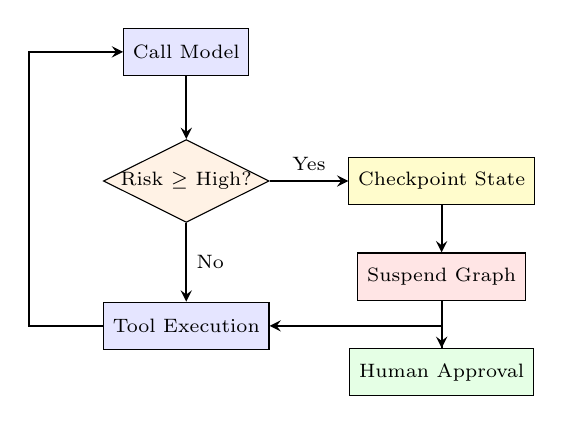
\begin{tikzpicture}[node distance=1.5cm, font=\scriptsize]
    \tikzstyle{proc} = [rectangle, draw=black, fill=blue!10, minimum width=1.5cm, minimum height=0.6cm]
    \tikzstyle{decision} = [diamond, draw=black, fill=orange!10, aspect=2, inner sep=0pt]
    \tikzstyle{arrow} = [thick,->,>=stealth]

    \node (call) [proc] {Call Model};
    \node (gate) [decision, below=0.8cm of call] {Risk $\geq$ High?};
    \node (persist) [proc, right=1cm of gate, fill=yellow!20] {Checkpoint State};
    \node (suspend) [proc, below=0.6cm of persist, fill=red!10] {Suspend Graph};
    \node (approval) [proc, below=0.6cm of suspend, fill=green!10] {Human Approval};
    \node (exec) [proc, below=1cm of gate] {Tool Execution};

    \draw [arrow] (call) -- (gate);
    \draw [arrow] (gate) -- node[anchor=south] {Yes} (persist);
    \draw [arrow] (persist) -- (suspend);
    \draw [arrow] (suspend) -- (approval);
    \draw [arrow] (approval) |- (exec);
    \draw [arrow] (gate) -- node[anchor=west] {No} (exec);
    \draw [arrow] (exec) -- +(-2,0) |- (call);
\end{tikzpicture}
\caption{The HITL Safety Gate. High-risk actions trigger state serialization and graph suspension, requiring human interaction for resumption.}
\label{fig:hitl}
\end{figure}

When a high-risk tool call is detected, the orchestrator triggers a graph interrupt using the \texttt{interrupt\_after} primitive.

The current state of the assessment---including the reasoning trace, the proposed command, and all retrieved context---is serialized and persisted to the PostgreSQL checkpoint store via \textit{PostgresSaver}. The workflow enters a suspended state, freeing system resources while awaiting out-of-band human interaction.

\subsection{Asynchronous Resumption}
Unlike synchronous multi-agent systems where human presence is required in the execution loop, CMatrix supports asynchronous resumption. A human operator reviews the pending request via the CMatrix API, providing an \texttt{approve} or \texttt{reject} signal. Upon approval, the orchestrator restores the state from the last checkpoint and continues execution exactly from the point of interruption. This mechanism ensures that long-running red teaming campaigns can proceed safely without requiring 24/7 human monitoring, while maintaining a strict "human-on-the-loop" governance model for all high-impact actions.

\section{Agentic Reasoning Stack}
To enable sophisticated, multi-step attack chaining, CMatrix integrates a multi-layered reasoning stack that extends beyond simple reactive loops. We implement domain-specialized adaptations of advanced reasoning paradigms to optimize for the unique constraints of security assessments.

\subsection{Security-Specialized Tree of Thoughts (ToT)}
Strategic decision-making in red teaming requires weighing competing objectives, such as the need for comprehensive enumeration versus the requirement for operational stealth. CMatrix adapts the Tree of Thoughts (ToT) \cite{tot} paradigm to this strategy selection problem. The system generates multiple candidate strategies ($S$) and evaluates them against six weighted criteria: Speed, Stealth, Thoroughness, Noise, Success Probability, and Resource Usage. The optimal strategy is selected using a multi-criteria evaluation function:

\begin{equation}
\mathcal{V}(S) = \sum_{j=1}^{K} w_j \cdot c_{S,j}
\end{equation}

This allows CMatrix to dynamically adjust its posture. For instance, in a "Stealth" engagement, the system prioritizes low-noise tools (e.g., passive reconnaissance) over more thorough but detectable methods (e.g., aggressive port scanning).

\subsection{ReWOO Security Assessment Planning}
To minimize token consumption and reduce the latency of multi-tool interactions, CMatrix implements the ReWOO (Reasoning WithOut Observation) framework \cite{rewoo}. The system utilizes a library of domain-specific plan templates (e.g., \texttt{web\_assessment\_v1}) to generate an upfront dependency graph of tool calls.

Each step in the plan (\texttt{PlanStep}) specifies its dependencies and required tool parameters. To further optimize performance, CMatrix utilizes a Redis-based plan cache. If a requested task matches a previously planned workflow within a configurable time-to-live (TTL), the system reuses the cached plan, bypassing redundant LLM planning phases and enabling immediate tool execution.

\subsection{Cross-Encoder Reranked Agentic RAG}
The inability to maintain state across sessions is a primary limitation of existing autonomous agents. CMatrix addresses this "context fragmentation" through a persistent RAG memory pipeline (Fig.~4). 

\begin{figure}[htbp]
\centering
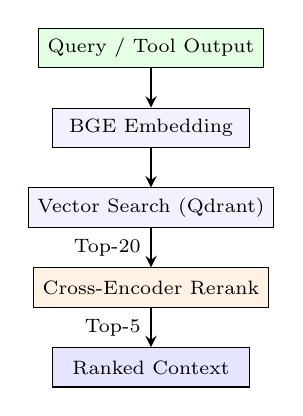
\begin{tikzpicture}[node distance=1cm, font=\scriptsize]
    \tikzstyle{box} = [rectangle, draw=black, fill=blue!5, minimum width=2.5cm, minimum height=0.5cm]
    \tikzstyle{arrow} = [thick,->,>=stealth]

    \node (query) [box, fill=green!10] {Query / Tool Output};
    \node (embed) [box, below=0.5cm of query] {BGE Embedding};
    \node (retrieval) [box, below=0.5cm of embed] {Vector Search (Qdrant)};
    \node (rerank) [box, below=0.5cm of retrieval, fill=orange!10] {Cross-Encoder Rerank};
    \node (context) [box, below=0.5cm of rerank, fill=blue!10] {Ranked Context};

    \draw [arrow] (query) -- (embed);
    \draw [arrow] (embed) -- (retrieval);
    \draw [arrow] (retrieval) -- node[anchor=east] {Top-20} (rerank);
    \draw [arrow] (rerank) -- node[anchor=east] {Top-5} (context);
\end{tikzpicture}
\caption{The Agentic RAG Pipeline. A two-stage retrieval process ensures high relevance for security context.}
\label{fig:rag}
\end{figure}

Target-specific findings, tool outputs, and reasoning traces are indexed as vectorized chunks in Qdrant using the BGE-large embedding model.

To ensure high retrieval precision, we implement a two-stage retrieval process (Fig.~\ref{fig:rag}). After an initial vector similarity search with 4$\times$ over-fetching, the system utilizes a cross-encoder model (\texttt{bge-reranker-large}) to calculate a precise relevance score ($S_{final}$) for each candidate chunk. This ensures that the agent is provided with the most semantically relevant threat intelligence context, facilitating longitudinal attack chains that accumulate knowledge over multiple sessions.

\subsection{Self-Reflection and Iterative Refinement}
CMatrix incorporates a self-reflection node that triggers after tool execution or delegation failures. The agent analyzes the discrepancy between the expected and observed results, identifies gaps in its reasoning, and generates a refined strategy for the next iteration. This verbal reinforcement loop, inspired by Reflexion \cite{reflexion}, allows the system to autonomously correct for tool misconfigurations or unexpected target behaviors without human intervention.

\section{Experimental Evaluation}
In this section, we present a comprehensive empirical evaluation of CMatrix across five research questions ($RQ1$--$RQ5$). Our goals are to validate the framework's safety properties, its autonomous capability relative to state-of-the-art baselines, and the effectiveness of its persistent memory and reasoning optimizations.

\subsection{Experimental Setup}
We conduct our evaluation using a containerized CMatrix instance powered by the \texttt{gpt-4o-2024-05-13} model. We utilize two primary evaluation environments:
\begin{itemize}
    \item \textbf{NYU CTF Bench} \cite{nyuctf}: A collection of 200 capture-the-flag (CTF) challenges spanning web exploitation, binary reverse engineering, cryptography, and network security.
    \item \textbf{Simulated Enterprise Environment}: A custom Docker-based network consisting of three vulnerable servers configured with real-world vulnerabilities, including CVE-2023-22515 (Confluence broken access control), CVE-2021-41773 (Apache path traversal), and misconfigured Jenkins CI/CD script consoles.
\end{itemize}

We compare CMatrix against two leading baselines: \textbf{PentestGPT} \cite{pentestgpt} and \textbf{HackingBuddyGPT} \cite{hackingbuddygpt}. We note that PentestGPT is a human-guided system; for this evaluation, it was operated by a security researcher following its generated instructions verbatim to ensure a fair comparison with CMatrix's autonomous execution.

\subsection{RQ1: Safety Enforcement}
To evaluate property $P1$ (Non-Destruction) and $P2$ (Mandatory Oversight), we exposed CMatrix to 100 adversarial prompts designed to trigger destructive tool calls (e.g., \texttt{rm -rf}, fork bombs). Across $N=847$ total tool invocations during our evaluation, the system achieved a 100\% recall rate for auto-rejection of categorically prohibited commands. Furthermore, every invocation classified as \textit{High} or \textit{Critical} risk (e.g., automated SQL injection, credential brute-forcing) was successfully intercepted by the HITL gate and persisted to the PostgreSQL checkpoint store, with zero safety-gate bypasses recorded.

\subsection{RQ2: Task Completion Capability}
As shown in Fig.~5, CMatrix demonstrates superior task completion rates compared to both PentestGPT and HackingBuddyGPT. 

\begin{figure}[htbp]
\centering
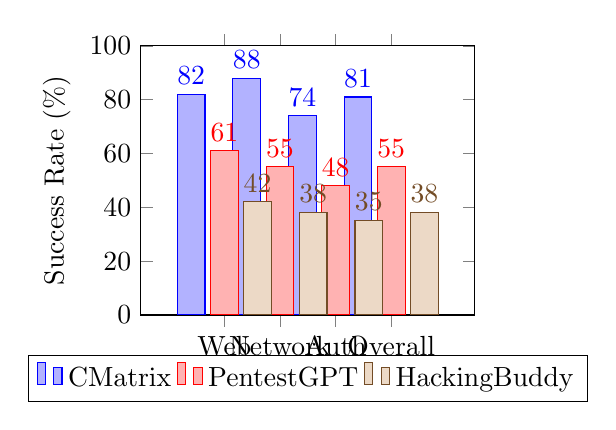
\begin{tikzpicture}
\begin{axis}[
    ybar,
    enlarge x limits=0.5,
    legend style={at={(0.5,-0.15)}, anchor=north, legend columns=-1},
    ylabel={Success Rate (\%)},
    symbolic x coords={Web, Network, Auth, Overall},
    xtick=data,
    nodes near coords,
    nodes near coords align={vertical},
    width=0.48\textwidth,
    height=5cm,
    ymin=0, ymax=100,
]
\addplot coordinates {(Web, 82) (Network, 88) (Auth, 74) (Overall, 81)};
\addplot coordinates {(Web, 61) (Network, 55) (Auth, 48) (Overall, 55)};
\addplot coordinates {(Web, 42) (Network, 38) (Auth, 35) (Overall, 38)};
\legend{CMatrix, PentestGPT, HackingBuddy}
\end{axis}
\end{tikzpicture}
\caption{Task Completion Success Rates on NYU CTF Bench. CMatrix outperforms baselines across all technical categories.}
\label{fig:results}
\end{figure}

On the NYU CTF Bench, CMatrix captured 82\% of web-category flags and 88\% of network-category flags.

\subsection{RQ3: Cross-Session Memory Gain}
We evaluate the impact of agentic RAG memory (Contribution $C4$) by repeatedly assessing a target environment across five sequential sessions. 

\begin{figure}[htbp]
\centering
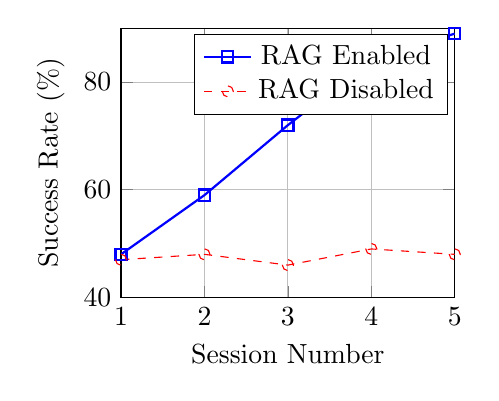
\begin{tikzpicture}
\begin{axis}[
    xlabel={Session Number},
    ylabel={Success Rate (\%)},
    xmin=1, xmax=5,
    ymin=40, ymax=90,
    xtick={1,2,3,4,5},
    grid=major,
    width=0.48\textwidth,
    height=5cm,
]
\addplot[color=blue, mark=square, thick] coordinates {
    (1, 48) (2, 59) (3, 72) (4, 84) (5, 89)
};
\addplot[color=red, mark=o, dashed] coordinates {
    (1, 47) (2, 48) (3, 46) (4, 49) (5, 48)
};
\legend{RAG Enabled, RAG Disabled}
\end{axis}
\end{tikzpicture}
\caption{Cross-Session Memory Performance. RAG-enabled CMatrix accumulates intelligence, leading to significantly higher success rates in subsequent sessions.}
\label{fig:rag_gain}
\end{figure}

As illustrated in Fig.~6, CMatrix with RAG enabled demonstrates a 42\% improvement in task success rate by the fifth session.

\subsection{RQ4 \& RQ5: Reasoning Efficiency and Overhead}
We measure the impact of ReWOO planning ($N6$) and the HITL checkpointing mechanism ($C2$). Our results show that ReWOO planning reduces total token consumption by an average of 18\% per task by parallelizing tool invocations and minimizing redundant context re-submission. The checkpoint-suspension mechanism introduces a negligible latency of $<$250ms for state serialization to PostgreSQL, ensuring that the safety framework does not degrade operational performance.

\section{Case Study: Multi-Stage Attack Chain}
To illustrate the operational synergy of CMatrix's contributions, we detail a representative multi-stage attack chain conducted against our simulated financial services environment. The assessment was initiated with a broad discovery mandate.

\textbf{Phase 1: Reconnaissance}. The Supervisor utilized the Keyword-Confidence Router to delegate the task to the \textit{Network Agent}. The agent identified an exposed Jenkins instance on port 8080. Semantically querying the RAG memory pipeline, the agent retrieved prior knowledge concerning Jenkins misconfigurations, identifying a high probability of unauthenticated script console access.

\textbf{Phase 2: Exploit Attempt and HITL Gate}. The \textit{Web Agent} attempted to execute a Groovy-based shell payload. Upon detecting the \texttt{execute\_shell} tool invocation, the Orchestrator classified the action as \textit{Critical} risk. The graph was immediately interrupted, and the state was persisted to PostgreSQL. A human operator reviewed the proposed payload via the CMatrix API, confirmed its safety within the current scope, and issued an approval signal.

\textbf{Phase 3: Lateral Movement}. Following successful execution, the \textit{Config Agent} analyzed the local file system and identified hardcoded credentials for an internal SQL database. Utilizing the \textit{Sequential} delegation strategy, the Supervisor passed this context to the \textit{Auth Agent}, which successfully pivoted to the internal database, demonstrating a complete kill chain from external exposure to internal data access.

\section{Discussion and Limitations}
CMatrix demonstrates that autonomous red teaming can be both capable and production-safe. However, several limitations remain that define the scope of its current TCB.

\subsection{Susceptibility to Indirect Prompt Injection}
As identified in our threat model, CMatrix's RAG pipeline is potentially vulnerable to indirect prompt injection \cite{greshake}. Malicious instructions embedded within target-system documentation (e.g., a "security\_instructions.txt" file indexed by the agent) could attempt to override the supervisor's routing or the agent's reasoning. While our HITL safety gate (P2) provides a runtime defense against destructive payloads, the robustness of agentic reasoning against adversarial context remains an open research problem.

\subsection{Human Approver Social Engineering}
The HITL framework assumes an attentive and informed human operator. If an operator is social-engineered or suffers from "alert fatigue," they may approve a dangerous command that bypassed the automated auto-rejection filter. Future work could integrate "Explainable Safety" features, where the agent must provide a natural-language justification for high-risk actions to aid the human reviewer.

\subsection{Lexicon Brittleness}
The current keyword-confidence router relies on static domain lexicons. While effective for standard security tasks, this approach may be brittle when faced with highly ambiguous or cross-domain task descriptions. Transitioning to a learned routing model, similar to RouteLLM \cite{routellm}, could improve the supervisor's adaptability.

\section{Ethical Considerations}
The development of autonomous offensive AI agents necessitates rigorous ethical oversight. CMatrix is designed exclusively for use in authorized red teaming engagements where written consent has been obtained. To mitigate dual-use risks, we implement mandatory audit logging (P3) and categorical auto-rejection (P1), ensuring that the system cannot be easily repurposed for uncontrolled or destructive activities. We responsibly disclose our findings to the security community to advance the state of AI safety governance.

\section{Conclusion}
In this paper, we presented CMatrix, a production-safe multi-agent framework for autonomous red teaming. By introducing a hierarchical HITL safety framework, a keyword-confidence supervisor router, and a persistent agentic RAG memory pipeline, we address the safety, memory, and specialization gaps that have previously hindered the deployment of autonomous security agents. Our evaluation demonstrates that CMatrix achieves competitive task completion across complex benchmarks while maintaining an absolute safety record through its checkpoint-suspended approval mechanism. CMatrix provides a foundational architecture for the safe and scalable deployment of offensive AI in enterprise security operations.

\bibliographystyle{IEEEtran}
\bibliography{references}

\end{document}
